\documentclass[twoside]{book}

% Packages required by doxygen
\usepackage{calc}
\usepackage{doxygen}
\usepackage{graphicx}
\usepackage[utf8]{inputenc}
\usepackage{makeidx}
\usepackage{multicol}
\usepackage{multirow}
\usepackage{textcomp}
\usepackage[table]{xcolor}

% NLS support packages
\usepackage{polski}
\usepackage[T1]{fontenc}

% Font selection
\usepackage[T1]{fontenc}
\usepackage{mathptmx}
\usepackage[scaled=.90]{helvet}
\usepackage{courier}
\usepackage{amssymb}
\usepackage{sectsty}
\renewcommand{\familydefault}{\sfdefault}
\allsectionsfont{%
  \fontseries{bc}\selectfont%
  \color{darkgray}%
}
\renewcommand{\DoxyLabelFont}{%
  \fontseries{bc}\selectfont%
  \color{darkgray}%
}

% Page & text layout
\usepackage{geometry}
\geometry{%
  a4paper,%
  top=2.5cm,%
  bottom=2.5cm,%
  left=2.5cm,%
  right=2.5cm%
}
\tolerance=750
\hfuzz=15pt
\hbadness=750
\setlength{\emergencystretch}{15pt}
\setlength{\parindent}{0cm}
\setlength{\parskip}{0.2cm}
\makeatletter
\renewcommand{\paragraph}{%
  \@startsection{paragraph}{4}{0ex}{-1.0ex}{1.0ex}{%
    \normalfont\normalsize\bfseries\SS@parafont%
  }%
}
\renewcommand{\subparagraph}{%
  \@startsection{subparagraph}{5}{0ex}{-1.0ex}{1.0ex}{%
    \normalfont\normalsize\bfseries\SS@subparafont%
  }%
}
\makeatother

% Headers & footers
\usepackage{fancyhdr}
\pagestyle{fancyplain}
\fancyhead[LE]{\fancyplain{}{\bfseries\thepage}}
\fancyhead[CE]{\fancyplain{}{}}
\fancyhead[RE]{\fancyplain{}{\bfseries\leftmark}}
\fancyhead[LO]{\fancyplain{}{\bfseries\rightmark}}
\fancyhead[CO]{\fancyplain{}{}}
\fancyhead[RO]{\fancyplain{}{\bfseries\thepage}}
\fancyfoot[LE]{\fancyplain{}{}}
\fancyfoot[CE]{\fancyplain{}{}}
\fancyfoot[RE]{\fancyplain{}{\bfseries\scriptsize Wygenerowano Śr, 18 mar 2015 08\-:07\-:00 dla Podstawowe struktury danych programem Doxygen }}
\fancyfoot[LO]{\fancyplain{}{\bfseries\scriptsize Wygenerowano Śr, 18 mar 2015 08\-:07\-:00 dla Podstawowe struktury danych programem Doxygen }}
\fancyfoot[CO]{\fancyplain{}{}}
\fancyfoot[RO]{\fancyplain{}{}}
\renewcommand{\footrulewidth}{0.4pt}
\renewcommand{\chaptermark}[1]{%
  \markboth{#1}{}%
}
\renewcommand{\sectionmark}[1]{%
  \markright{\thesection\ #1}%
}

% Indices & bibliography
\usepackage{natbib}
\usepackage[titles]{tocloft}
\setcounter{tocdepth}{3}
\setcounter{secnumdepth}{5}
\makeindex

% Hyperlinks (required, but should be loaded last)
\usepackage{ifpdf}
\ifpdf
  \usepackage[pdftex,pagebackref=true]{hyperref}
\else
  \usepackage[ps2pdf,pagebackref=true]{hyperref}
\fi
\hypersetup{%
  colorlinks=true,%
  linkcolor=blue,%
  citecolor=blue,%
  unicode%
}

% Custom commands
\newcommand{\clearemptydoublepage}{%
  \newpage{\pagestyle{empty}\cleardoublepage}%
}


%===== C O N T E N T S =====

\begin{document}

% Titlepage & ToC
\hypersetup{pageanchor=false}
\pagenumbering{roman}
\begin{titlepage}
\vspace*{7cm}
\begin{center}%
{\Large Podstawowe struktury danych \\[1ex]\large 1 }\\
\vspace*{1cm}
{\large Wygenerowano przez Doxygen 1.8.6}\\
\vspace*{0.5cm}
{\small Śr, 18 mar 2015 08:07:00}\\
\end{center}
\end{titlepage}
\clearemptydoublepage
\tableofcontents
\clearemptydoublepage
\pagenumbering{arabic}
\hypersetup{pageanchor=true}

%--- Begin generated contents ---
\chapter{Sprawozdanie}
\label{_sprawozdanie}
\hypertarget{_sprawozdanie}{}
\begin{DoxyDate}{Data}
11.\-03.\-2015r. 
\end{DoxyDate}
\begin{DoxyVersion}{Wersja}
0.\-1 
\end{DoxyVersion}
\hypertarget{_sprawozdanie_Zadanie}{}\section{Zadanie}\label{_sprawozdanie_Zadanie}
Celem ćwiczenia było stworzenie programu benchmarkującego , który dla wybranych danych będzie zliczał średni czas wykonania dowolnego algorytmu ( w tym przypadku mnożenia elementów tablicy przez 2). Należało również stworzyć program generujący losowe liczby.\hypertarget{_sprawozdanie_Wyniki}{}\section{Wyniki}\label{_sprawozdanie_Wyniki}
Dla dziesięciu milionów liczb program zwraca 7 danych wyjściowych ( zgodnie z algorytmem 10$^\wedge$n , gdzie n jest równocześnie ilością zwracanych czasów oraz maxymalną liczbą danych dla jakiej przeprowadzany był test

Na podstawie otrzymanych danych mamy \-:


\begin{DoxyImageNoCaption}
  \mbox{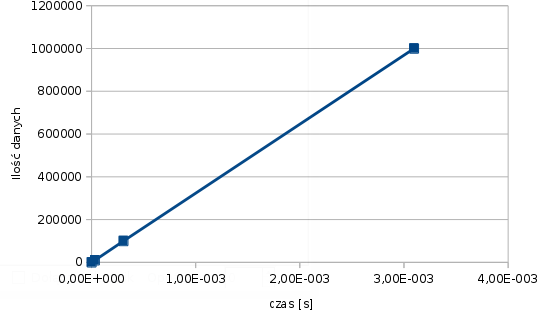
\includegraphics{1.jpg}}
\end{DoxyImageNoCaption}
\hypertarget{_sprawozdanie_Podsumowanie}{}\section{Podsumowanie}\label{_sprawozdanie_Podsumowanie}
Wykres dodany do dokumentacji z niewiadomych względów nie jest wyświetlany poprawnie ( dodano sprawozdanie również w formacie pdf). Zgodnie z przewidywaniami złożoność obliczeniowa jest liniowa , jedyną rzeczą która zwraca uwagę jest fakt iż czas wykonania jednej operacji jest dłuższy od czasu wykonania 10 operacji. Dla wiekszej ilości danych wyniki są poprawne Wydaje się , że zbyt mało danych jest obecnych w środkowej częsci wykresu co powinno być zostać zmienione w celu poprawy jakości odbioru wykresu ( dla charakterystyki liniowej jest to akurat bez znaczenia ale .np dla logarytmicznej było by widoczne ). 
\chapter{Indeks hierarchiczny}
\section{Hierarchia klas}
Ta lista dziedziczenia posortowana jest z grubsza, choć nie całkowicie, alfabetycznie\-:\begin{DoxyCompactList}
\item \contentsline{section}{benchmark}{\pageref{classbenchmark}}{}
\begin{DoxyCompactList}
\item \contentsline{section}{tabx2}{\pageref{classtabx2}}{}
\end{DoxyCompactList}
\end{DoxyCompactList}

\chapter{Indeks klas}
\section{Lista klas}
Tutaj znajdują się klasy, struktury, unie i interfejsy wraz z ich krótkimi opisami\-:\begin{DoxyCompactList}
\item\contentsline{section}{\hyperlink{classbenchmark}{benchmark} }{\pageref{classbenchmark}}{}
\item\contentsline{section}{\hyperlink{classtabx2}{tabx2} }{\pageref{classtabx2}}{}
\end{DoxyCompactList}

\chapter{Indeks plików}
\section{Lista plików}
Tutaj znajduje się lista wszystkich plików z ich krótkimi opisami\-:\begin{DoxyCompactList}
\item\contentsline{section}{\hyperlink{benchmark_8cpp}{benchmark.\-cpp} \\*Deklaracja funkzji z klasy Benchmark }{\pageref{benchmark_8cpp}}{}
\item\contentsline{section}{\hyperlink{benchmark_8hh}{benchmark.\-hh} \\*Definicja klasy Benchmark }{\pageref{benchmark_8hh}}{}
\item\contentsline{section}{\hyperlink{generator_8cpp}{generator.\-cpp} \\*Deklaracja funckji generujacej liczby losowe }{\pageref{generator_8cpp}}{}
\item\contentsline{section}{\hyperlink{generator_8hh}{generator.\-hh} \\*Definicja generatora liczb losowych }{\pageref{generator_8hh}}{}
\item\contentsline{section}{\hyperlink{main_8cpp}{main.\-cpp} }{\pageref{main_8cpp}}{}
\item\contentsline{section}{\hyperlink{tabx2_8cpp}{tabx2.\-cpp} \\*Deklaracja klasy \hyperlink{classtabx2}{tabx2} }{\pageref{tabx2_8cpp}}{}
\item\contentsline{section}{\hyperlink{tabx2_8hh}{tabx2.\-hh} \\*Definicja klasy \hyperlink{classtabx2}{tabx2} }{\pageref{tabx2_8hh}}{}
\end{DoxyCompactList}

\chapter{Dokumentacja klas}
\hypertarget{classbenchmark}{\section{Dokumentacja klasy benchmark}
\label{classbenchmark}\index{benchmark@{benchmark}}
}


{\ttfamily \#include $<$benchmark.\-hh$>$}



Diagram dziedziczenia dla benchmark\nopagebreak
\begin{figure}[H]
\begin{center}
\leavevmode
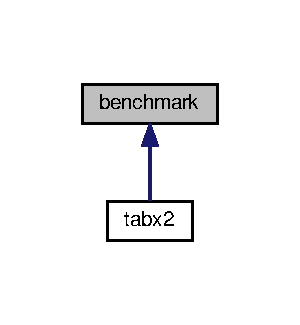
\includegraphics[width=144pt]{classbenchmark__inherit__graph}
\end{center}
\end{figure}
\subsection*{Metody publiczne}
\begin{DoxyCompactItemize}
\item 
void \hyperlink{classbenchmark_a23e508cd746c10ba8a650965673aa839}{analyze} (int repeat, int data\-\_\-amount)
\begin{DoxyCompactList}\small\item\em Metoda analyze zlicza czas wykonywania funkcji \hyperlink{classbenchmark_a698d333f815e6e12c0817b1dfee56e99}{test()} \par
 Uwaga! do poprawnego działania wymagane jest posiadanie programu gnuplot. \end{DoxyCompactList}\end{DoxyCompactItemize}
\subsection*{Metody prywatne}
\begin{DoxyCompactItemize}
\item 
virtual void \hyperlink{classbenchmark_a698d333f815e6e12c0817b1dfee56e99}{test} (int length)=0
\begin{DoxyCompactList}\small\item\em Metoda test funkcja wirtualna , której czas działania ma być aproksymowany przez metoda \hyperlink{classbenchmark_a23e508cd746c10ba8a650965673aa839}{analyze()} \end{DoxyCompactList}\end{DoxyCompactItemize}


\subsection{Opis szczegółowy}


Definicja w linii 11 pliku benchmark.\-hh.



\subsection{Dokumentacja funkcji składowych}
\hypertarget{classbenchmark_a23e508cd746c10ba8a650965673aa839}{\index{benchmark@{benchmark}!analyze@{analyze}}
\index{analyze@{analyze}!benchmark@{benchmark}}
\subsubsection[{analyze}]{\setlength{\rightskip}{0pt plus 5cm}void benchmark\-::analyze (
\begin{DoxyParamCaption}
\item[{int}]{repeat, }
\item[{int}]{data\-\_\-amount}
\end{DoxyParamCaption}
)}}\label{classbenchmark_a23e508cd746c10ba8a650965673aa839}
Metoda analyze zlicza czas fukcji \hyperlink{classbenchmark_a698d333f815e6e12c0817b1dfee56e99}{test()} \par
Przykład wywołania funkcji \-: \par
analyze(100,7) -\/$>$ Przeprowadza analize czesu trwania funkcji \hyperlink{classbenchmark_a698d333f815e6e12c0817b1dfee56e99}{test()} dla 1 miliona danych , każdy czas trwania funkcji jest ustalany na podstawie średniej arytmetycznej ze 100 prób.


\begin{DoxyParams}[1]{Parametry}
\mbox{\tt in}  & {\em repeat} & -\/ ilość powtórzeń testu \\
\hline
\mbox{\tt in}  & {\em data\-\_\-amount} & -\/ ilosc wynikowych danych podawana jako potega liczby 10 \\
\hline
\end{DoxyParams}
\begin{DoxyReturn}{Zwraca}
plik.\-dat z czasami poszczegolnych pomiarow oraz ilosc testowanych danych oraz plik plot.\-png bedacy graficznym przedstawieniem danych na wykresie 
\end{DoxyReturn}


Definicja w linii 15 pliku benchmark.\-cpp.



Oto graf wywołań dla tej funkcji\-:\nopagebreak
\begin{figure}[H]
\begin{center}
\leavevmode
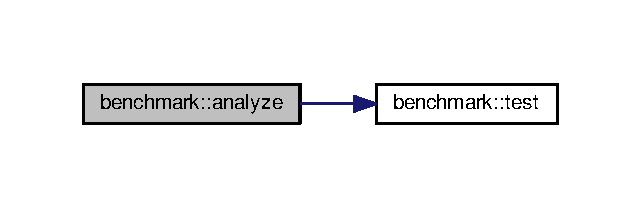
\includegraphics[width=308pt]{classbenchmark_a23e508cd746c10ba8a650965673aa839_cgraph}
\end{center}
\end{figure}




Oto graf wywoływań tej funkcji\-:\nopagebreak
\begin{figure}[H]
\begin{center}
\leavevmode
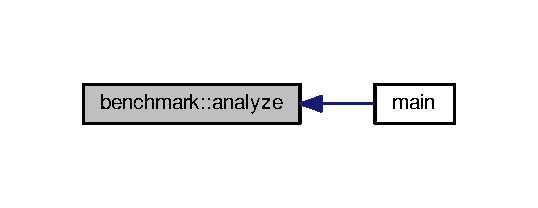
\includegraphics[width=258pt]{classbenchmark_a23e508cd746c10ba8a650965673aa839_icgraph}
\end{center}
\end{figure}


\hypertarget{classbenchmark_a698d333f815e6e12c0817b1dfee56e99}{\index{benchmark@{benchmark}!test@{test}}
\index{test@{test}!benchmark@{benchmark}}
\subsubsection[{test}]{\setlength{\rightskip}{0pt plus 5cm}virtual void benchmark\-::test (
\begin{DoxyParamCaption}
\item[{int}]{length}
\end{DoxyParamCaption}
)\hspace{0.3cm}{\ttfamily [private]}, {\ttfamily [pure virtual]}}}\label{classbenchmark_a698d333f815e6e12c0817b1dfee56e99}


Implementowany w \hyperlink{classtabx2_a41eea5dffaea0a866db5c574129c0ee4}{tabx2}.



Oto graf wywoływań tej funkcji\-:\nopagebreak
\begin{figure}[H]
\begin{center}
\leavevmode
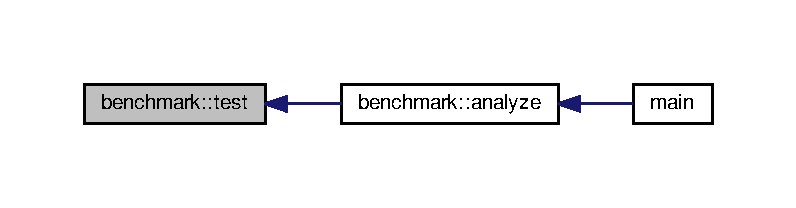
\includegraphics[width=350pt]{classbenchmark_a698d333f815e6e12c0817b1dfee56e99_icgraph}
\end{center}
\end{figure}




Dokumentacja dla tej klasy została wygenerowana z plików\-:\begin{DoxyCompactItemize}
\item 
\hyperlink{benchmark_8hh}{benchmark.\-hh}\item 
\hyperlink{benchmark_8cpp}{benchmark.\-cpp}\end{DoxyCompactItemize}

\hypertarget{classtabx2}{\section{Dokumentacja klasy tabx2}
\label{classtabx2}\index{tabx2@{tabx2}}
}


{\ttfamily \#include $<$tabx2.\-hh$>$}



Diagram dziedziczenia dla tabx2\nopagebreak
\begin{figure}[H]
\begin{center}
\leavevmode
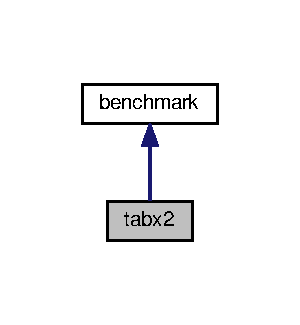
\includegraphics[width=144pt]{classtabx2__inherit__graph}
\end{center}
\end{figure}


Diagram współpracy dla tabx2\-:\nopagebreak
\begin{figure}[H]
\begin{center}
\leavevmode
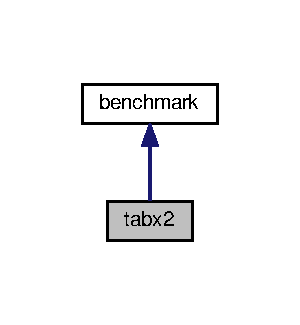
\includegraphics[width=144pt]{classtabx2__coll__graph}
\end{center}
\end{figure}
\subsection*{Metody publiczne}
\begin{DoxyCompactItemize}
\item 
void \hyperlink{classtabx2_a41eea5dffaea0a866db5c574129c0ee4}{test} (int length)
\begin{DoxyCompactList}\small\item\em Tworzy tablice alokowana dynamicznie o pojemnosci wybranej przez uzytkownika , umozliwia wykonywanie mnozenia przez 2 wszystkich elementow tablicy. \end{DoxyCompactList}\item 
\hyperlink{classtabx2_a68be0fc6ed6ce41d56011a6f5bad1b00}{tabx2} (int \hyperlink{classtabx2_a9a6db4f12091baed13f8bad9b9538766}{size})
\begin{DoxyCompactList}\small\item\em Konstruktor paramteryczny. \end{DoxyCompactList}\item 
\hyperlink{classtabx2_a6e259fbc3e5791ae3a11df988a8369c0}{$\sim$tabx2} ()
\begin{DoxyCompactList}\small\item\em Zwykly destruktor. \end{DoxyCompactList}\end{DoxyCompactItemize}
\subsection*{Atrybuty prywatne}
\begin{DoxyCompactItemize}
\item 
int \hyperlink{classtabx2_a9a6db4f12091baed13f8bad9b9538766}{size}
\begin{DoxyCompactList}\small\item\em Rozmiar tablicy. \end{DoxyCompactList}\item 
int $\ast$ \hyperlink{classtabx2_ae3ee40d58c1d3dc6a80c34ca63d337e9}{tab}
\begin{DoxyCompactList}\small\item\em Wskaznik na tablice przechowujaca dane. \end{DoxyCompactList}\end{DoxyCompactItemize}


\subsection{Opis szczegółowy}


Definicja w linii 14 pliku tabx2.\-hh.



\subsection{Dokumentacja konstruktora i destruktora}
\hypertarget{classtabx2_a68be0fc6ed6ce41d56011a6f5bad1b00}{\index{tabx2@{tabx2}!tabx2@{tabx2}}
\index{tabx2@{tabx2}!tabx2@{tabx2}}
\subsubsection[{tabx2}]{\setlength{\rightskip}{0pt plus 5cm}tabx2\-::tabx2 (
\begin{DoxyParamCaption}
\item[{int}]{size}
\end{DoxyParamCaption}
)}}\label{classtabx2_a68be0fc6ed6ce41d56011a6f5bad1b00}
Konstruktor wczytujacy okreslona ilosc danych i alokujacy je dynamicznie 
\begin{DoxyParams}[1]{Parametry}
\mbox{\tt in}  & {\em size} & -\/ dlugosc tablice \\
\hline
\end{DoxyParams}


Definicja w linii 21 pliku tabx2.\-cpp.

\hypertarget{classtabx2_a6e259fbc3e5791ae3a11df988a8369c0}{\index{tabx2@{tabx2}!$\sim$tabx2@{$\sim$tabx2}}
\index{$\sim$tabx2@{$\sim$tabx2}!tabx2@{tabx2}}
\subsubsection[{$\sim$tabx2}]{\setlength{\rightskip}{0pt plus 5cm}tabx2\-::$\sim$tabx2 (
\begin{DoxyParamCaption}
{}
\end{DoxyParamCaption}
)}}\label{classtabx2_a6e259fbc3e5791ae3a11df988a8369c0}


Definicja w linii 41 pliku tabx2.\-cpp.



\subsection{Dokumentacja funkcji składowych}
\hypertarget{classtabx2_a41eea5dffaea0a866db5c574129c0ee4}{\index{tabx2@{tabx2}!test@{test}}
\index{test@{test}!tabx2@{tabx2}}
\subsubsection[{test}]{\setlength{\rightskip}{0pt plus 5cm}void tabx2\-::test (
\begin{DoxyParamCaption}
\item[{int}]{length}
\end{DoxyParamCaption}
)\hspace{0.3cm}{\ttfamily [virtual]}}}\label{classtabx2_a41eea5dffaea0a866db5c574129c0ee4}
Mnozy okreslona ilosc danych przez 2 
\begin{DoxyParams}[1]{Parametry}
\mbox{\tt in}  & {\em length} & -\/ ilosc danych do przemnozenia \\
\hline
\end{DoxyParams}


Implementuje \hyperlink{classbenchmark_a698d333f815e6e12c0817b1dfee56e99}{benchmark}.



Definicja w linii 13 pliku tabx2.\-cpp.



\subsection{Dokumentacja atrybutów składowych}
\hypertarget{classtabx2_a9a6db4f12091baed13f8bad9b9538766}{\index{tabx2@{tabx2}!size@{size}}
\index{size@{size}!tabx2@{tabx2}}
\subsubsection[{size}]{\setlength{\rightskip}{0pt plus 5cm}int tabx2\-::size\hspace{0.3cm}{\ttfamily [private]}}}\label{classtabx2_a9a6db4f12091baed13f8bad9b9538766}


Definicja w linii 22 pliku tabx2.\-hh.

\hypertarget{classtabx2_ae3ee40d58c1d3dc6a80c34ca63d337e9}{\index{tabx2@{tabx2}!tab@{tab}}
\index{tab@{tab}!tabx2@{tabx2}}
\subsubsection[{tab}]{\setlength{\rightskip}{0pt plus 5cm}int$\ast$ tabx2\-::tab\hspace{0.3cm}{\ttfamily [private]}}}\label{classtabx2_ae3ee40d58c1d3dc6a80c34ca63d337e9}


Definicja w linii 25 pliku tabx2.\-hh.



Dokumentacja dla tej klasy została wygenerowana z plików\-:\begin{DoxyCompactItemize}
\item 
\hyperlink{tabx2_8hh}{tabx2.\-hh}\item 
\hyperlink{tabx2_8cpp}{tabx2.\-cpp}\end{DoxyCompactItemize}

\chapter{Dokumentacja plików}
\hypertarget{benchmark_8cpp}{\section{Dokumentacja pliku benchmark.\-cpp}
\label{benchmark_8cpp}\index{benchmark.\-cpp@{benchmark.\-cpp}}
}


Deklaracja funkzji z klasy Benchmark.  


{\ttfamily \#include \char`\"{}benchmark.\-hh\char`\"{}}\\*
Wykres zależności załączania dla benchmark.\-cpp\-:\nopagebreak
\begin{figure}[H]
\begin{center}
\leavevmode
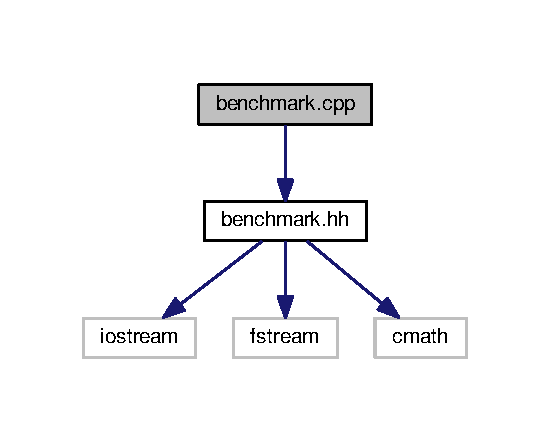
\includegraphics[width=330pt]{benchmark_8cpp__incl}
\end{center}
\end{figure}

\hypertarget{benchmark_8hh}{\section{Dokumentacja pliku benchmark.\-hh}
\label{benchmark_8hh}\index{benchmark.\-hh@{benchmark.\-hh}}
}


Definicja klasy Benchmark.  


{\ttfamily \#include $<$iostream$>$}\\*
{\ttfamily \#include $<$fstream$>$}\\*
{\ttfamily \#include $<$cmath$>$}\\*
{\ttfamily \#include \char`\"{}stdlib.\-h\char`\"{}}\\*
Wykres zależności załączania dla benchmark.\-hh\-:\nopagebreak
\begin{figure}[H]
\begin{center}
\leavevmode
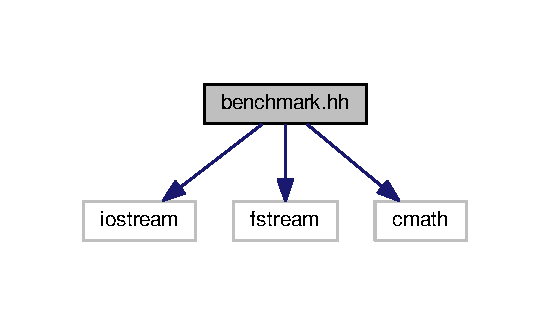
\includegraphics[width=330pt]{benchmark_8hh__incl}
\end{center}
\end{figure}
Ten wykres pokazuje, które pliki bezpośrednio lub pośrednio załączają ten plik\-:\nopagebreak
\begin{figure}[H]
\begin{center}
\leavevmode
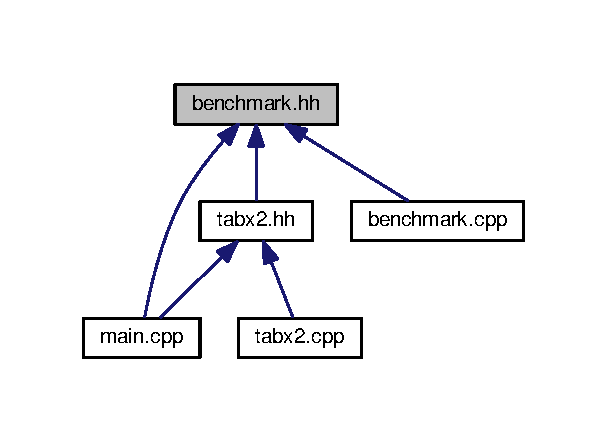
\includegraphics[width=291pt]{benchmark_8hh__dep__incl}
\end{center}
\end{figure}
\subsection*{Komponenty}
\begin{DoxyCompactItemize}
\item 
class \hyperlink{classbenchmark}{benchmark}
\end{DoxyCompactItemize}

\hypertarget{generator_8cpp}{}\section{generator.\+cpp File Reference}
\label{generator_8cpp}\index{generator.\+cpp@{generator.\+cpp}}


Deklaracja funckji generujacej liczby losowe.  


{\ttfamily \#include \char`\"{}generator.\+hh\char`\"{}}\\*
Include dependency graph for generator.\+cpp\+:\nopagebreak
\begin{figure}[H]
\begin{center}
\leavevmode
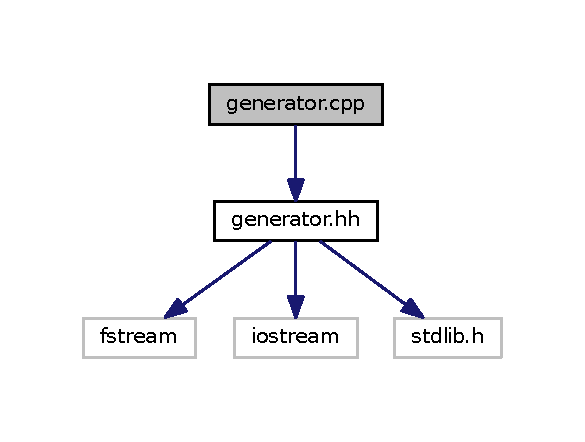
\includegraphics[width=281pt]{d0/d00/generator_8cpp__incl}
\end{center}
\end{figure}
\subsection*{Functions}
\begin{DoxyCompactItemize}
\item 
bool \hyperlink{generator_8cpp_a6c501967035e575874570ef71d23f3af}{data\+\_\+generator} (int data\+\_\+amount)
\begin{DoxyCompactList}\small\item\em Generuje liczby losowe. \end{DoxyCompactList}\end{DoxyCompactItemize}


\subsection{Detailed Description}
Deklaracja funckji generujacej liczby losowe. 



Definition in file \hyperlink{generator_8cpp_source}{generator.\+cpp}.



\subsection{Function Documentation}
\hypertarget{generator_8cpp_a6c501967035e575874570ef71d23f3af}{}\index{generator.\+cpp@{generator.\+cpp}!data\+\_\+generator@{data\+\_\+generator}}
\index{data\+\_\+generator@{data\+\_\+generator}!generator.\+cpp@{generator.\+cpp}}
\subsubsection[{data\+\_\+generator}]{\setlength{\rightskip}{0pt plus 5cm}bool data\+\_\+generator (
\begin{DoxyParamCaption}
\item[{int}]{data\+\_\+amount}
\end{DoxyParamCaption}
)}\label{generator_8cpp_a6c501967035e575874570ef71d23f3af}


Generuje liczby losowe. 

Funkcja generuje naturalne liczby losowe z przedziału 0-\/100, ktore nastepnie sa zapisywane do pliku random\+\_\+data.\+dat 
\begin{DoxyParams}[1]{Parameters}
\mbox{\tt in}  & {\em data\+\_\+amount} & -\/ ilosc liczb wynikowych ktore chcemy uzyskac \\
\hline
\end{DoxyParams}


Definition at line \hyperlink{generator_8cpp_source_l00009}{9} of file \hyperlink{generator_8cpp_source}{generator.\+cpp}.


\hypertarget{generator_8hh}{\section{Dokumentacja pliku generator.\-hh}
\label{generator_8hh}\index{generator.\-hh@{generator.\-hh}}
}


Definicja generatora liczb losowych.  


{\ttfamily \#include $<$fstream$>$}\\*
{\ttfamily \#include $<$iostream$>$}\\*
{\ttfamily \#include $<$stdlib.\-h$>$}\\*
Wykres zależności załączania dla generator.\-hh\-:\nopagebreak
\begin{figure}[H]
\begin{center}
\leavevmode
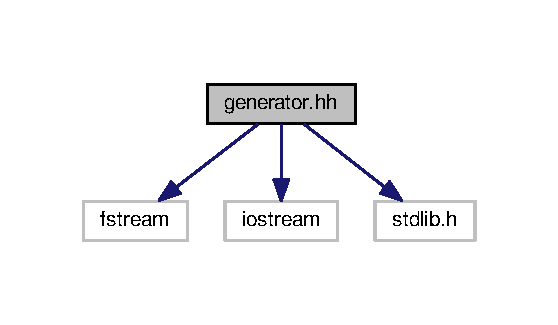
\includegraphics[width=268pt]{generator_8hh__incl}
\end{center}
\end{figure}
Ten wykres pokazuje, które pliki bezpośrednio lub pośrednio załączają ten plik\-:\nopagebreak
\begin{figure}[H]
\begin{center}
\leavevmode
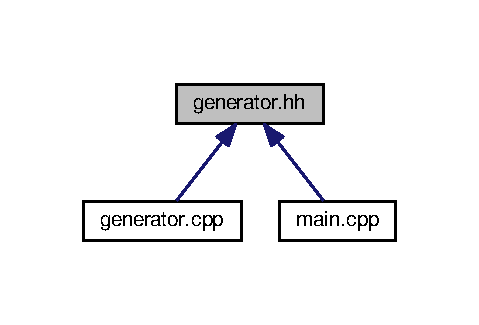
\includegraphics[width=230pt]{generator_8hh__dep__incl}
\end{center}
\end{figure}
\subsection*{Funkcje}
\begin{DoxyCompactItemize}
\item 
bool \hyperlink{generator_8hh_a6c501967035e575874570ef71d23f3af}{data\-\_\-generator} (int data\-\_\-amount)
\begin{DoxyCompactList}\small\item\em Generuje liczby losowe. \end{DoxyCompactList}\end{DoxyCompactItemize}


\subsection{Dokumentacja funkcji}
\hypertarget{generator_8hh_a6c501967035e575874570ef71d23f3af}{\index{generator.\-hh@{generator.\-hh}!data\-\_\-generator@{data\-\_\-generator}}
\index{data\-\_\-generator@{data\-\_\-generator}!generator.hh@{generator.\-hh}}
\subsubsection[{data\-\_\-generator}]{\setlength{\rightskip}{0pt plus 5cm}bool data\-\_\-generator (
\begin{DoxyParamCaption}
\item[{int}]{data\-\_\-amount}
\end{DoxyParamCaption}
)}}\label{generator_8hh_a6c501967035e575874570ef71d23f3af}
Funkcja generuje naturalne liczby losowe z przedziału 0-\/100, ktore nastepnie sa zapisywane do pliku random\-\_\-data.\-dat 
\begin{DoxyParams}[1]{Parametry}
\mbox{\tt in}  & {\em data\-\_\-amount} & -\/ ilosc liczb wynikowych ktore chcemy uzyskac \\
\hline
\end{DoxyParams}


Definicja w linii 9 pliku generator.\-cpp.


\hypertarget{main_8cpp}{\section{Dokumentacja pliku main.\-cpp}
\label{main_8cpp}\index{main.\-cpp@{main.\-cpp}}
}
{\ttfamily \#include \char`\"{}tabx2.\-hh\char`\"{}}\\*
{\ttfamily \#include \char`\"{}benchmark.\-hh\char`\"{}}\\*
{\ttfamily \#include \char`\"{}generator.\-hh\char`\"{}}\\*
Wykres zależności załączania dla main.\-cpp\-:\nopagebreak
\begin{figure}[H]
\begin{center}
\leavevmode
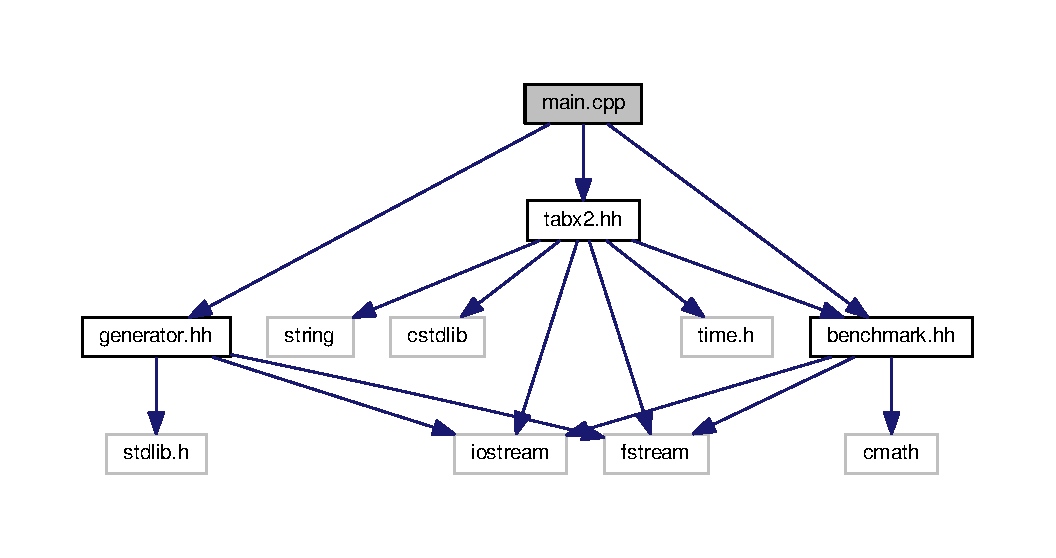
\includegraphics[width=350pt]{main_8cpp__incl}
\end{center}
\end{figure}
\subsection*{Funkcje}
\begin{DoxyCompactItemize}
\item 
int \hyperlink{main_8cpp_ae66f6b31b5ad750f1fe042a706a4e3d4}{main} ()
\end{DoxyCompactItemize}


\subsection{Dokumentacja funkcji}
\hypertarget{main_8cpp_ae66f6b31b5ad750f1fe042a706a4e3d4}{\index{main.\-cpp@{main.\-cpp}!main@{main}}
\index{main@{main}!main.cpp@{main.\-cpp}}
\subsubsection[{main}]{\setlength{\rightskip}{0pt plus 5cm}int main (
\begin{DoxyParamCaption}
{}
\end{DoxyParamCaption}
)}}\label{main_8cpp_ae66f6b31b5ad750f1fe042a706a4e3d4}


Definicja w linii 6 pliku main.\-cpp.



Oto graf wywołań dla tej funkcji\-:
\nopagebreak
\begin{figure}[H]
\begin{center}
\leavevmode
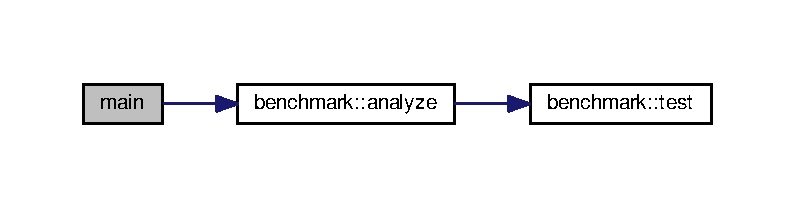
\includegraphics[width=350pt]{main_8cpp_ae66f6b31b5ad750f1fe042a706a4e3d4_cgraph}
\end{center}
\end{figure}



\hypertarget{strona_8dox}{}\section{strona.\+dox File Reference}
\label{strona_8dox}\index{strona.\+dox@{strona.\+dox}}

\hypertarget{tabx2_8cpp}{}\section{tabx2.\+cpp File Reference}
\label{tabx2_8cpp}\index{tabx2.\+cpp@{tabx2.\+cpp}}


Deklaracja klasy main.  


{\ttfamily \#include \char`\"{}tabx2.\+hh\char`\"{}}\\*
Include dependency graph for tabx2.\+cpp\+:\nopagebreak
\begin{figure}[H]
\begin{center}
\leavevmode
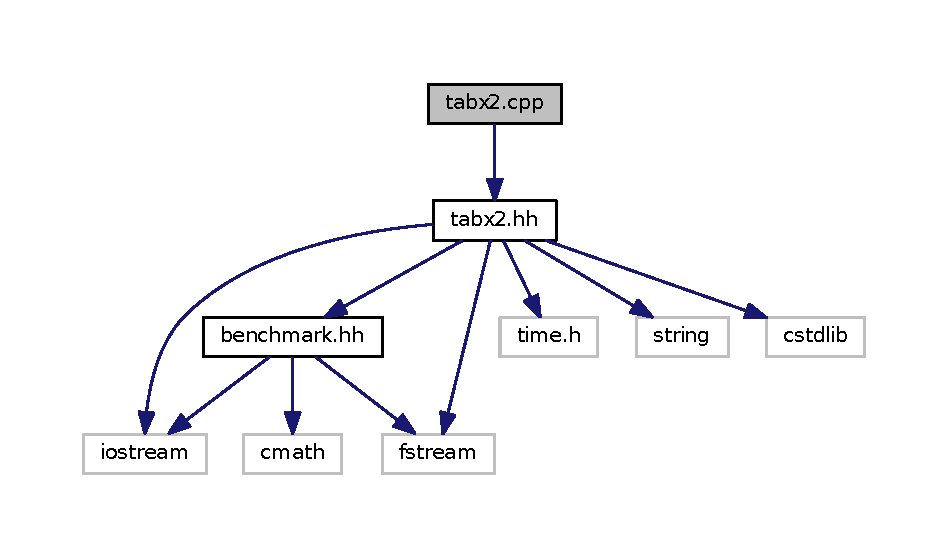
\includegraphics[width=350pt]{d5/d0d/tabx2_8cpp__incl}
\end{center}
\end{figure}


\subsection{Detailed Description}
Deklaracja klasy main. 



Definition in file \hyperlink{tabx2_8cpp_source}{tabx2.\+cpp}.


\hypertarget{tabx2_8hh}{\section{Dokumentacja pliku tabx2.\-hh}
\label{tabx2_8hh}\index{tabx2.\-hh@{tabx2.\-hh}}
}


Definicja klasy \hyperlink{classtabx2}{tabx2}.  


{\ttfamily \#include $<$iostream$>$}\\*
{\ttfamily \#include $<$time.\-h$>$}\\*
{\ttfamily \#include $<$string$>$}\\*
{\ttfamily \#include $<$fstream$>$}\\*
{\ttfamily \#include $<$cstdlib$>$}\\*
{\ttfamily \#include \char`\"{}benchmark.\-hh\char`\"{}}\\*
Wykres zależności załączania dla tabx2.\-hh\-:\nopagebreak
\begin{figure}[H]
\begin{center}
\leavevmode
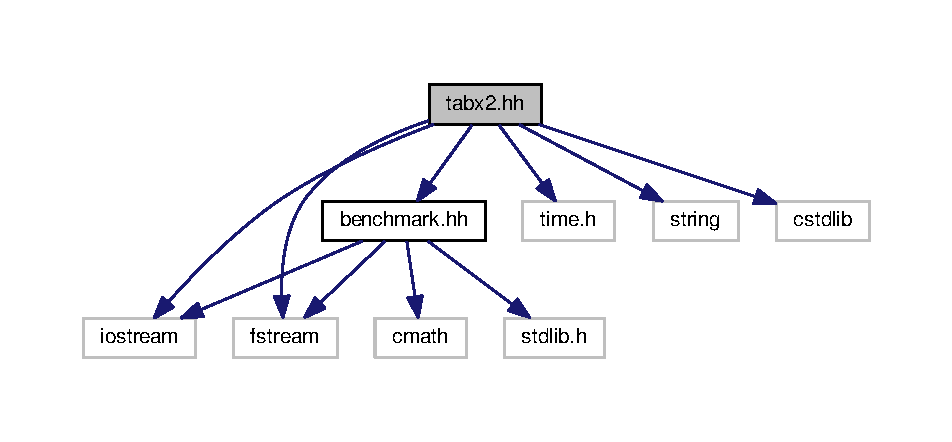
\includegraphics[width=350pt]{tabx2_8hh__incl}
\end{center}
\end{figure}
Ten wykres pokazuje, które pliki bezpośrednio lub pośrednio załączają ten plik\-:\nopagebreak
\begin{figure}[H]
\begin{center}
\leavevmode
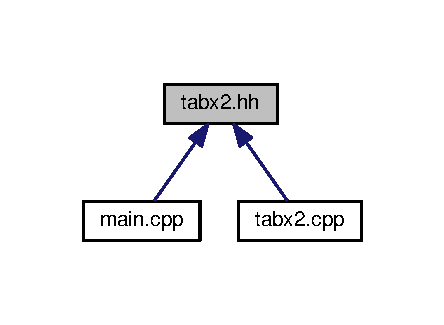
\includegraphics[width=213pt]{tabx2_8hh__dep__incl}
\end{center}
\end{figure}
\subsection*{Komponenty}
\begin{DoxyCompactItemize}
\item 
class \hyperlink{classtabx2}{tabx2}
\end{DoxyCompactItemize}
\subsection*{Definicje}
\begin{DoxyCompactItemize}
\item 
\#define \hyperlink{tabx2_8hh_ab76bf9329c796034d3ea1300008f135e}{T\-A\-B\-X2\-\_\-\-H\-H}
\end{DoxyCompactItemize}


\subsection{Opis szczegółowy}
Plik zawiera definicję klasy tabx2.\-Modeluje glowne pojecia zwiazane z programem 

Definicja w pliku \hyperlink{tabx2_8hh_source}{tabx2.\-hh}.



\subsection{Dokumentacja definicji}
\hypertarget{tabx2_8hh_ab76bf9329c796034d3ea1300008f135e}{\index{tabx2.\-hh@{tabx2.\-hh}!T\-A\-B\-X2\-\_\-\-H\-H@{T\-A\-B\-X2\-\_\-\-H\-H}}
\index{T\-A\-B\-X2\-\_\-\-H\-H@{T\-A\-B\-X2\-\_\-\-H\-H}!tabx2.hh@{tabx2.\-hh}}
\subsubsection[{T\-A\-B\-X2\-\_\-\-H\-H}]{\setlength{\rightskip}{0pt plus 5cm}\#define T\-A\-B\-X2\-\_\-\-H\-H}}\label{tabx2_8hh_ab76bf9329c796034d3ea1300008f135e}


Definicja w linii 2 pliku tabx2.\-hh.


%--- End generated contents ---

% Index
\newpage
\phantomsection
\addcontentsline{toc}{chapter}{Indeks}
\printindex

\end{document}
